% Copyright 2004 by Till Tantau <tantau@users.sourceforge.net>.
%
% In principle, this file can be redistributed and/or modified under
% the terms of the GNU Public License, version 2.
%
% However, this file is supposed to be a template to be modified
% for your own needs. For this reason, if you use this file as a
% template and not specifically distribute it as part of a another
% package/program, I grant the extra permission to freely copy and
% modify this file as you see fit and even to delete this copyright
% notice. 

\documentclass[aspectratio=169]{beamer}
%\documentclass{beamer}

\setbeamersize{text margin left=5mm, text margin right=5mm}


\defbeamertemplate{headline}{my header}{%
\vskip1pt%
\makebox[0pt][l]{\,\insertshortauthor}%
\hspace*{\fill}\insertshorttitle/\insertshortsubtitle\hspace*{\fill}%
\llap{\insertpagenumber/\insertpresentationendpage\,}
}
\setbeamertemplate{headline}[my header]

\let\olditem\item
\renewcommand{\item}{\setlength{\itemsep}{\fill}\olditem}

\usepackage{soul}
\usepackage{tkz-euclide}
\usetikzlibrary{calc}
\usepackage[]{algorithm2e}
\usepackage{changepage}
\usepackage{amssymb}
\usepackage{xcolor}
\usepackage{mathtools}
\usepackage{tcolorbox}
\usepackage{tikz}
\usepackage{tikz-3dplot}
\usepackage[export]{adjustbox}
\usepackage{tabu}

% \usepackage{courierten}
% \renewcommand*\familydefault{\ttdefault} %% Only if the base font of the document is to be typewriter style
% \usepackage[T1]{fontenc}

% \usepackage[math]{cellspace}
% \cellspacetoplimit 4pt
% \cellspacebottomlimit 4pt
%\usetikzlibrary{arrows.meta}

%\setbeamertemplate{itemize items}{-}

%\usepackage{helvet}
\usefonttheme{professionalfonts} % using non standard fonts for beamer
%\usefonttheme{serif} % default family is serif
%\usepackage{fontspec}
%\setmainfont{Liberation Serif}

% There are many different themes available for Beamer. A comprehensive
% list with examples is given here:
% http://deic.uab.es/~iblanes/beamer_gallery/index_by_theme.html
% You can uncomment the themes below if you would like to use a different
% one:
%\usetheme{AnnArbor}
%\usetheme{Antibes}
%\usetheme{Bergen}
%\usetheme{Berkeley}
%\usetheme{Berlin}
%\usetheme{Boadilla}
%\usetheme{boxes}
%\usetheme{CambridgeUS}
%\usetheme{Copenhagen}
%\usetheme{Darmstadt}
%\usetheme{default}
%\usetheme{Frankfurt}
%\usetheme{Goettingen}
%\usetheme{Hannover}
%\usetheme{Ilmenau}
%\usetheme{JuanLesPins}
%\usetheme{Luebeck}
%\usetheme{Madrid}
%\usetheme{Malmoe}
%\usetheme{Marburg}
%\usetheme{Montpellier}
%\usetheme{PaloAlto}
%\usetheme{Pittsburgh}
%\usetheme{Rochester}
%\usetheme{Singapore}
%\usetheme{Szeged}
%\usetheme{Warsaw}


\def\mf{\ensuremath\mathbf}
\def\mb{\ensuremath\mathbb}
\def\mc{\ensuremath\mathcal}
\def\lp{\ensuremath\left(}
\def\rp{\ensuremath\right)}
\def\lv{\ensuremath\left\lvert}
\def\rv{\ensuremath\right\rvert}
\def\lV{\ensuremath\left\lVert}
\def\rV{\ensuremath\right\rVert}
\def\lc{\ensuremath\left\{}
\def\rc{\ensuremath\right\}}
\def\ls{\ensuremath\left[}
\def\rs{\ensuremath\right]}
\def\bmx{\ensuremath\begin{bmatrix*}[r]}
\def\emx{\ensuremath\end{bmatrix*}}
\def\bmxc{\ensuremath\begin{bmatrix*}[c]}
\def\t{\lp t\rp}
\def\k{\ls k\rs}


\newcommand{\demoex}[2]{\onslide<#1->\begin{color}{black!60} #2 \end{color}}
\newcommand{\demoexc}[3]{\onslide<#1->\begin{color}{#2} #3 \end{color}}
\newcommand{\anim}[3]{\onslide<#1->{\begin{color}{#2!60} #3 \end{color}}}
\newcommand{\ct}[1]{\lp #1\rp}
\newcommand{\dt}[1]{\ls #1\rs}
\newcommand{\cols}[2]{\begin{columns}[#1] #2 \end{columns}}
\newcommand{\col}[2]{\begin{column}{#1} #2 \end{column}}

\newcommand{\xdownarrow}[1]{%
  {\left\downarrow\vbox to #1{}\right.\kern-\nulldelimiterspace}
}

\title{Introduction to Digital Signal Processing}

% A subtitle is optional and this may be deleted
\subtitle{Digital Filters}

\author{Sivakumar Balasubramanian}
% - Give the names in the same order as the appear in the paper.
% - Use the \inst{?} command only if the authors have different
%   affiliation.

\institute[Christian Medical College] % (optional, but mostly needed)
{
  \inst{}%
  Department of Bioengineering\\
  Christian Medical College, Bagayam\\
  Vellore 632002
}
% - Use the \inst command only if there are several affiliations.
% - Keep it simple, no one is interested in your street address.

\date{}
% - Either use conference name or its abbreviation.
% - Not really informative to the audience, more for people (including
%   yourself) who are reading the slides online

\subject{Lecture slides on Introduction to DSP}
% This is only inserted into the PDF information catalog. Can be left
% out. 

% If you have a file called "university-logo-filename.xxx", where xxx
% is a graphic format that can be processed by latex or pdflatex,
% resp., then you can add a logo as follows:

% \pgfdeclareimage[height=0.5cm]{university-logo}{university-logo-filename}
% \logo{\pgfuseimage{university-logo}}

% Delete this, if you do not want the table of contents to pop up at
% the beginning of each subsection:
\AtBeginSubsection[]
{
  \begin{frame}<beamer>{Outline}
    \tableofcontents[currentsection,currentsubsection]
  \end{frame}
}

% Let's get started
\begin{document}

\begin{frame}
  \titlepage
\end{frame}


\begin{frame}[t]{LTI systems can be designed shape frequency spectrum}
Let $H$ be an LTI system,

\[ e^{j\Omega n} \mapsto \vert H\lp \Omega \rp \vert e^{j\Omega n + \arg H\lp \Omega\rp} \]

The amount of amplitude and phase modification of the input $e^{j\Omega n}$ is determined by the magntiude and phase of the value of the transfer function $H\lp \Omega \rp$.
\vspace{0.5cm}

The frequency response a discrete-time LTI system can be obtained from its impulse response or the difference equation describing the system,
\[ H\lp \Omega \rp = \sum_{n} h[n] e^{-j\Omega n} = \frac{\sum_{k=1}^M b_i z^{-k}}{\sum_{l=1}^N a_l z^{-k}}\bigg\vert_{z = e^{j\Omega}} \]

If we have a desired frequency response $H_d\lp \Omega \rp$, how do we choose the impulse response or the coefficients of the LTI system such that its frequency response $H\lp \Omega \rp$ is as close to $H_d\lp \Omega \rp$ as possible. 
\end{frame}


\begin{frame}[t]{Need for frequency selective filters}
  \begin{figure}
  \centering
  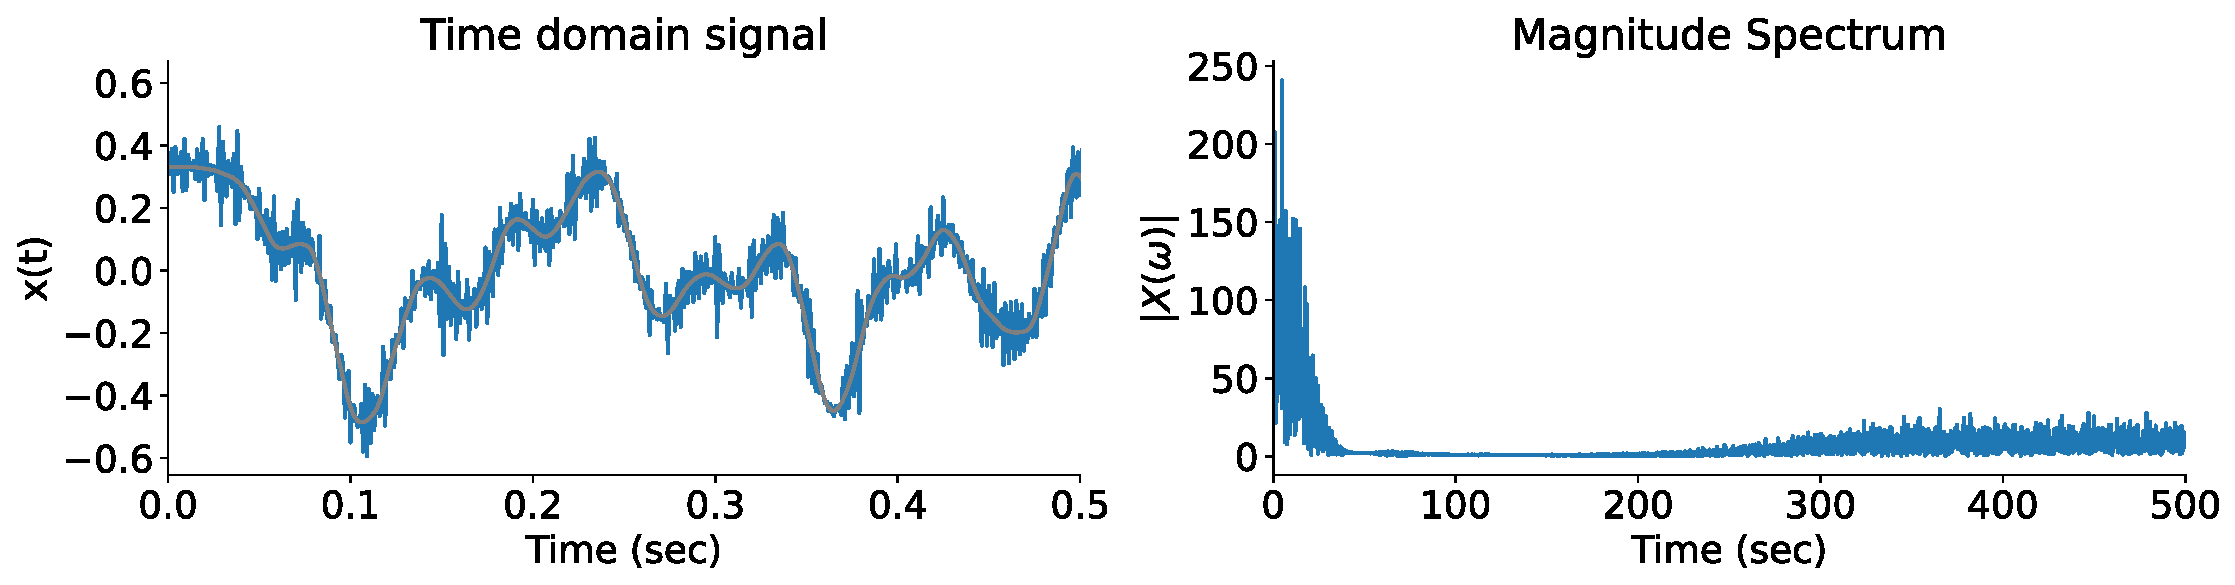
\includegraphics[width=1\textwidth]{img/example1.eps}
  \end{figure}
\end{frame}


\begin{frame}[t]{Ideal Filters}
  \begin{figure}
  \centering
  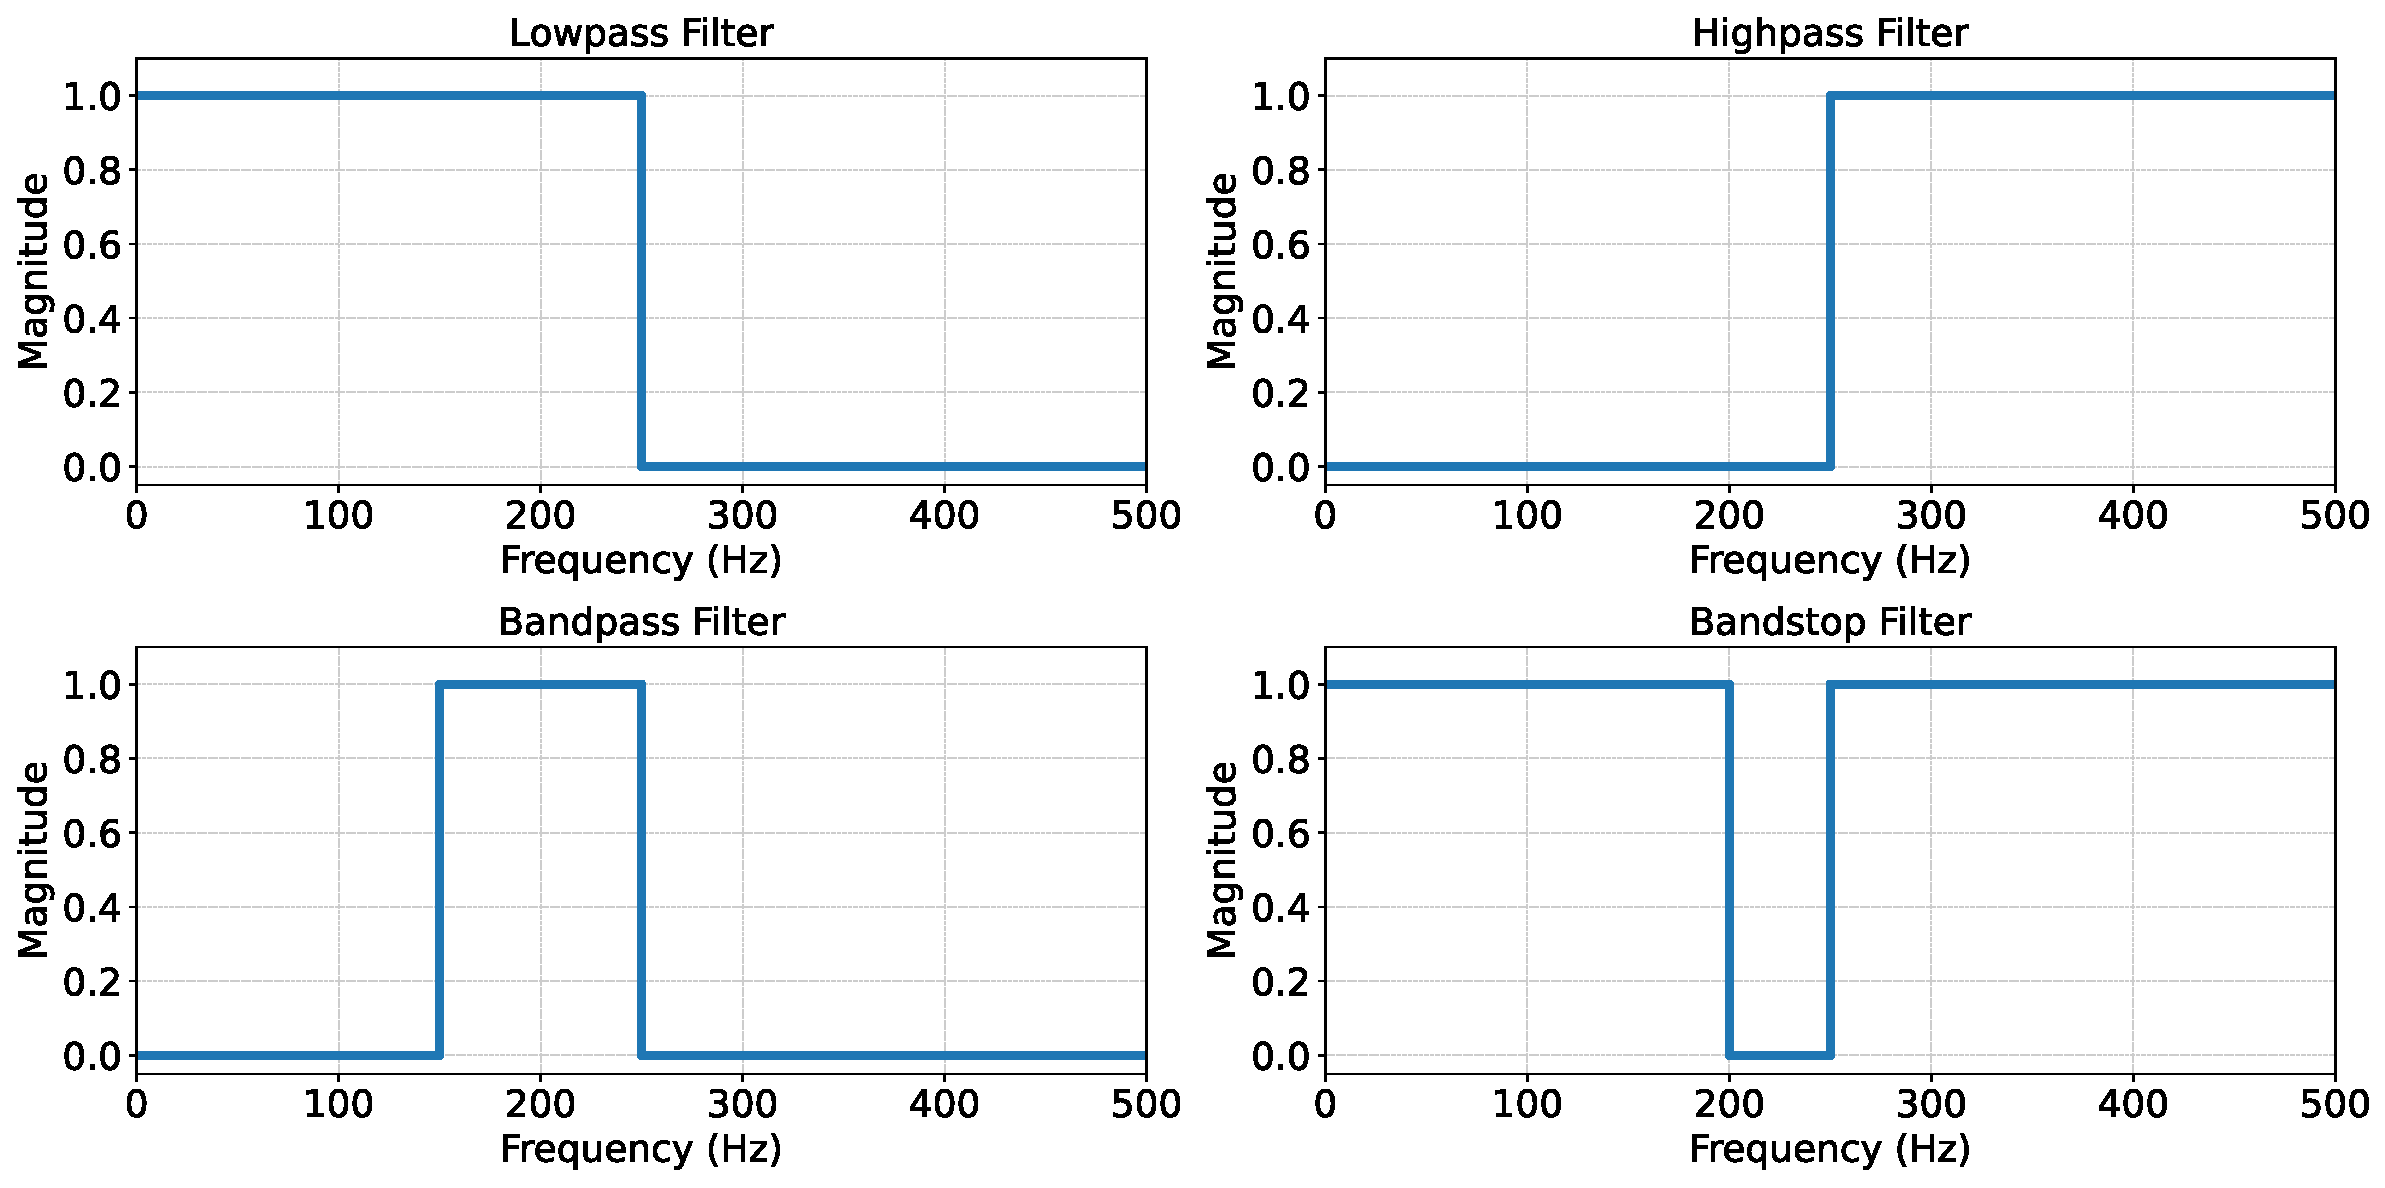
\includegraphics[width=1\textwidth]{img/idealfilts.eps}
  \end{figure}
\end{frame}


\begin{frame}[t]{Characteristics of Ideal Filter }
Consider the ideal lowpass filter, 
\[ H\lp \Omega \rp = \begin{cases} C\cdot e^{-j\omega n_0}, & \vert \Omega \vert \leq \Omega_c \\ 0, & \Omega_c < >\vert \Omega \vert \leq \pi \end{cases} \]

\[ \implies Y\lp \Omega \rp = X\lp \Omega \rp H\lp \Omega \rp = C X\lp \Omega \rp e^{-j\Omega n_0} \]
\vspace{0.5cm}

\begin{itemize}
  \item $C \implies $ Constant scaling of amplitude in the passband.
  \item $e^{j \Omega n_0} \implies $ Linear phase, which a constant time delay for all frequency components. 
\end{itemize}

\vspace{1cm}

But ideal filters are problematic!
\end{frame}


\begin{frame}[t]{Problems with ideal}
  Ideal filters are not physically realizable.
  \vspace{0.5cm}

  Consider the ideal lowpass filter, $H\lp \Omega \rp = \begin{cases} 1, & \vert \Omega \vert \leq \Omega_c \\ 0, & \Omega_c \vert \Omega \vert \leq \pi \end{cases}$. The inverse DTFT of $H\lp \Omega \rp$ will give us the following impulse response for the system,

  \[ h[n] = 2 \Omega_c \frac{\sin \Omega_c n}{\Omega_c n} \]

  This is non-causal, with $h[n]$ extending upto $-\infty$.
  \vspace{1cm}

  Physically realizable filters cannot have:
  \begin{itemize}
    \item Flat frequecny response over a continuous interval.
    \item Cannot have step transitions.
  \end{itemize}
\end{frame}


\begin{frame}[t]{Real Filter Specifications}
  \begin{figure}
  \centering
  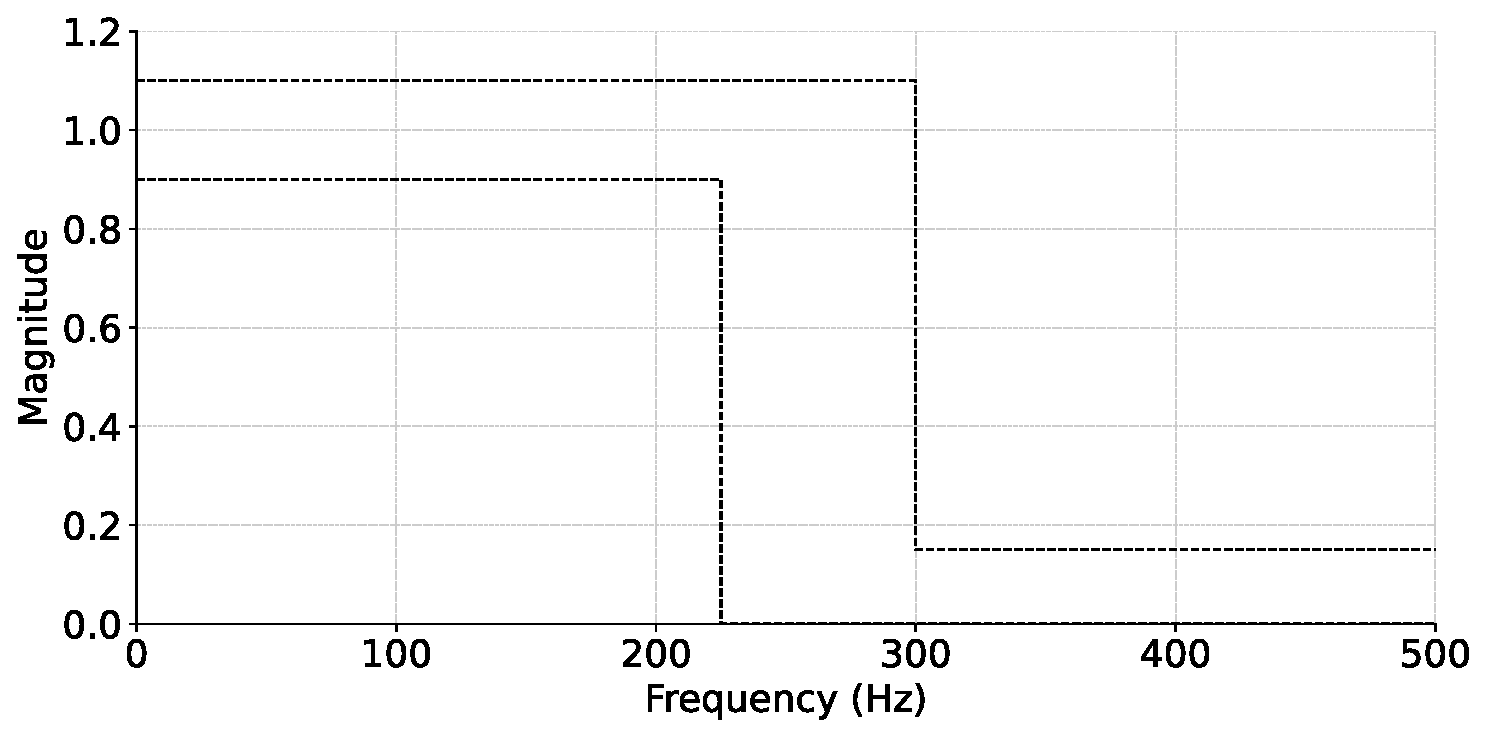
\includegraphics[width=0.9\textwidth]{img/filtspec.eps}
  \end{figure}
\end{frame}


\begin{frame}[t]{Real Filter Specifications}
\begin{Large}
  \[ \delta_1, \,\, \delta_2, \,\, f_p, \,\, f_s \longrightarrow H\lp \Omega \rp \longrightarrow \frac{\sum_{k=0}^M b_i z^{-k}}{1 + \sum_{l=1}^N a_l z^{-k}}\bigg\vert_{z = e^{j\Omega}} \]
\end{Large}

Parameters to be chosen for a filter: $N$, $M$, $\lp a_i \rp_{i=1}^N$, and $\lp b_i \rp_{i=0}^M$.

\[ H(z) = b_0 \frac{\prod_{k=1}^M \lp 1 - z_kz^{-1}\rp}{\prod_{k=1}^N \lp 1 - p_kz^{-1}\rp} \]

\begin{itemize}
  \item $\lp a_i \rp_{i=1}^N$ determine the \textbf{poles} of the transfer function $\lp p_i \rp_{i=1}^N \longrightarrow$ Can be used to \textbf{emphasize certain frequencies}.
  \item $\lp b_i \rp_{i=0}^M$ determine the \textbf{zeros} of the transfer function  $\lp z_i \rp_{i=1}^M \longrightarrow$ Can be used to \textbf{attenuate certain frequencies}.
\end{itemize}

Appropriate placement of the poles and zeros will allow us to obtain a frequency response that satisfies the given filter specifications.
\end{frame}


\begin{frame}[t]
  \frametitle{Pole-Zero Placement and Frequency Response}
  \begin{figure}
  \centering
  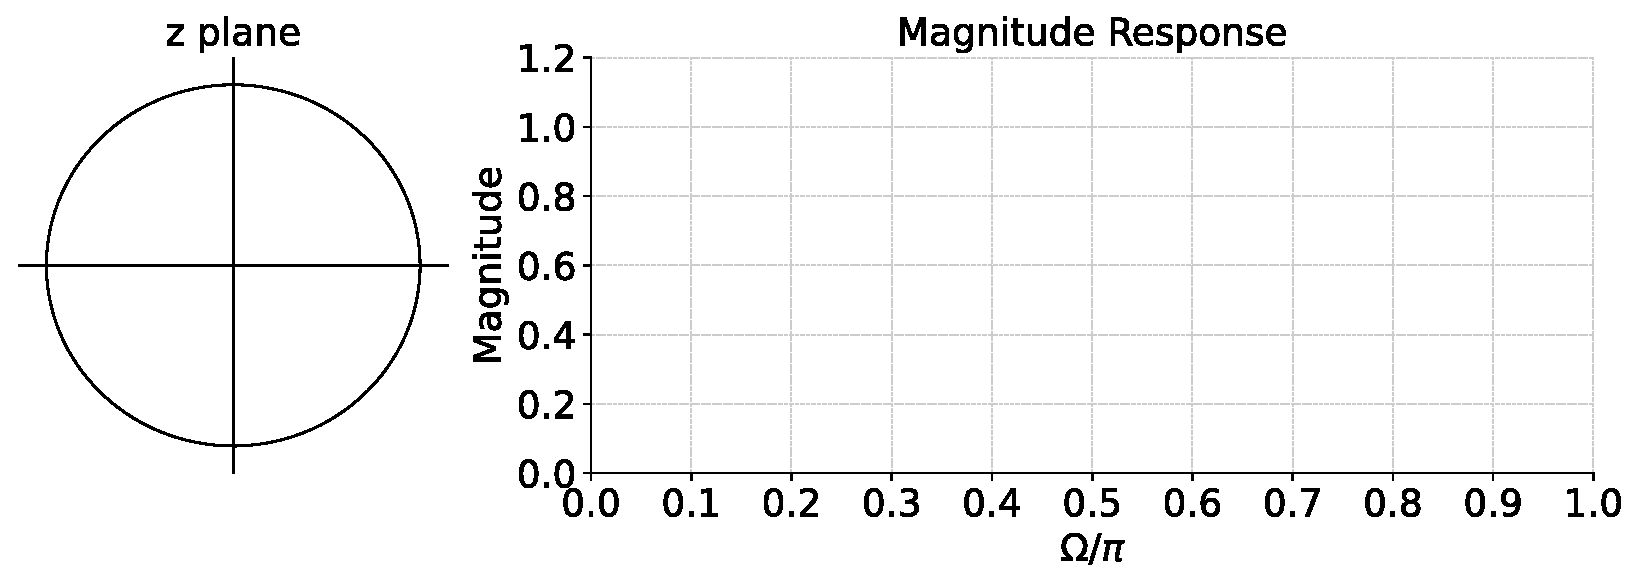
\includegraphics[width=0.7\textwidth]{img/freqpz.eps}
  \end{figure}

  \begin{figure}
  \centering
  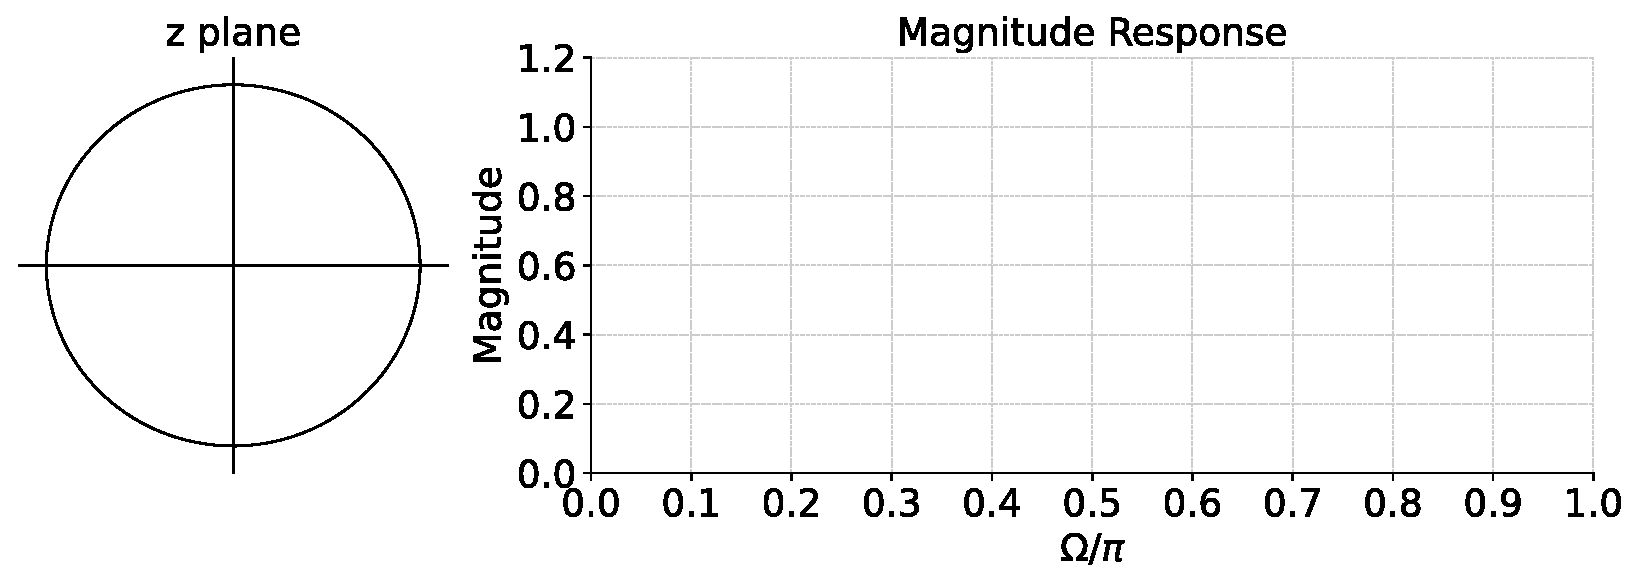
\includegraphics[width=0.7\textwidth]{img/freqpz.eps}
  \end{figure}
\end{frame}


\begin{frame}[t]
  \frametitle{Pole-Zero Placement and Frequency Response}
  Consider the two pole system,
  \[ H(z) = \frac{b_0}{1 - 2pz^{-1} + p^2z^{-2}} \]
  Determine $b_0$ and $p$ such that the frequency response,
   \[ H(\Omega = 0) = 1 \quad \text{and} \quad \big \vert H(\Omega = \frac{\pi}{2}) \big \vert = \frac{1}{\sqrt{2}} \]
\end{frame}


\begin{frame}[t]
  \frametitle{}
  
\end{frame}


\begin{frame}[t]
  \frametitle{Pole-Zero Placement and Frequency Response}
  Consider the two pole system,
  \[ H(z) = \frac{b_0}{1 - 2pz^{-1} + p^2z^{-2}} \]
  Determine $b_0$ and $p$ such that the frequency response,
   \[ H(\Omega = 0) = 1 \quad \text{and} \quad \big \vert H(\Omega = \frac{\pi}{4}) \big \vert = \frac{1}{\sqrt{2}} \]
\end{frame}


\begin{frame}[t]
  \frametitle{}
  
\end{frame}


\begin{frame}[t]
  \frametitle{Pole-Zero Placement and Frequency Response}

  \begin{figure}
  \centering
  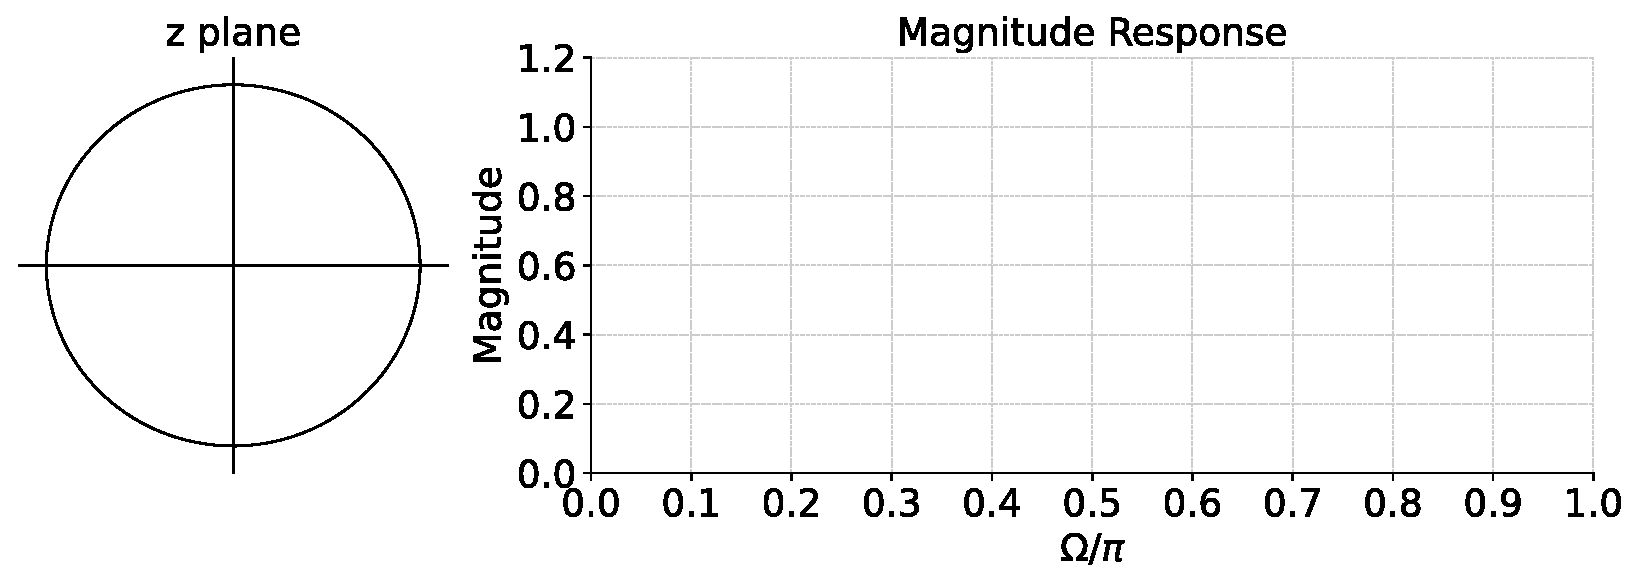
\includegraphics[width=0.7\textwidth]{img/freqpz.eps}
  \end{figure}

  \begin{figure}
  \centering
  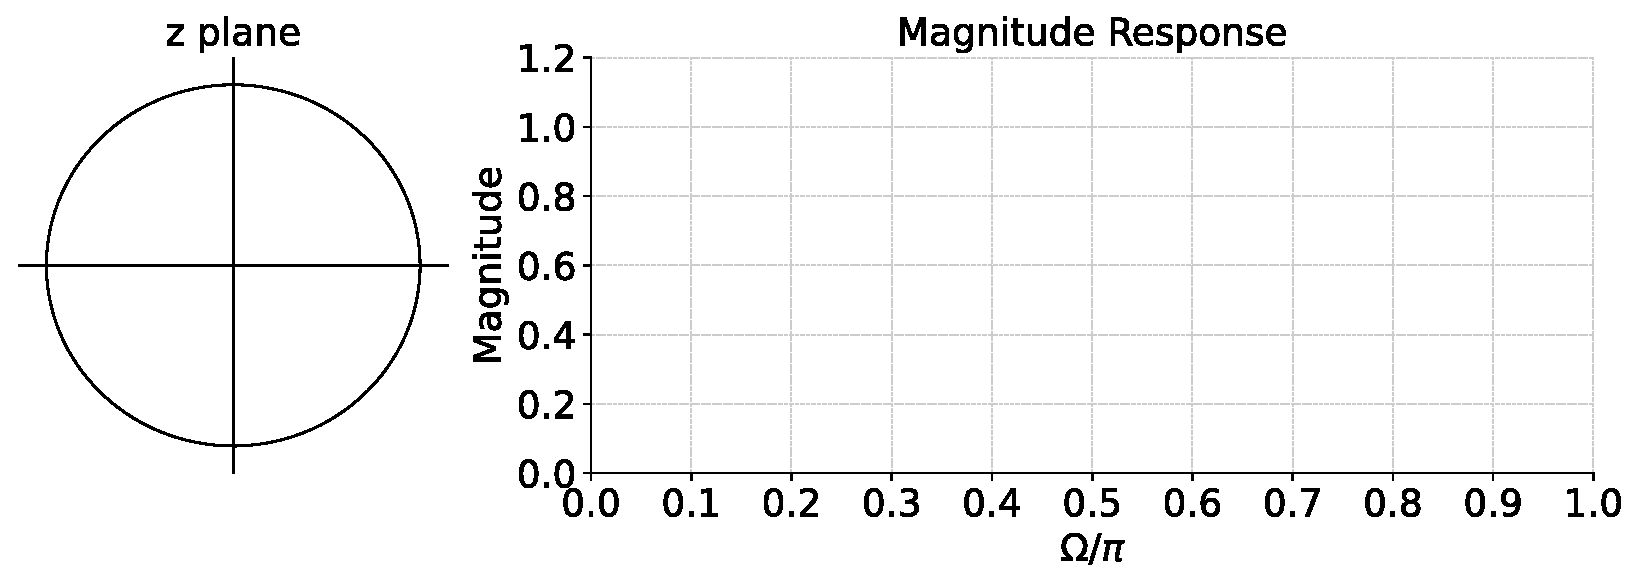
\includegraphics[width=0.7\textwidth]{img/freqpz.eps}
  \end{figure}
  
\end{frame}


\begin{frame}[t]
  \frametitle{}
  
\end{frame}


\begin{frame}[t]
  \frametitle{Pole-Zero Placement and Frequency Response}

  \begin{figure}
  \centering
  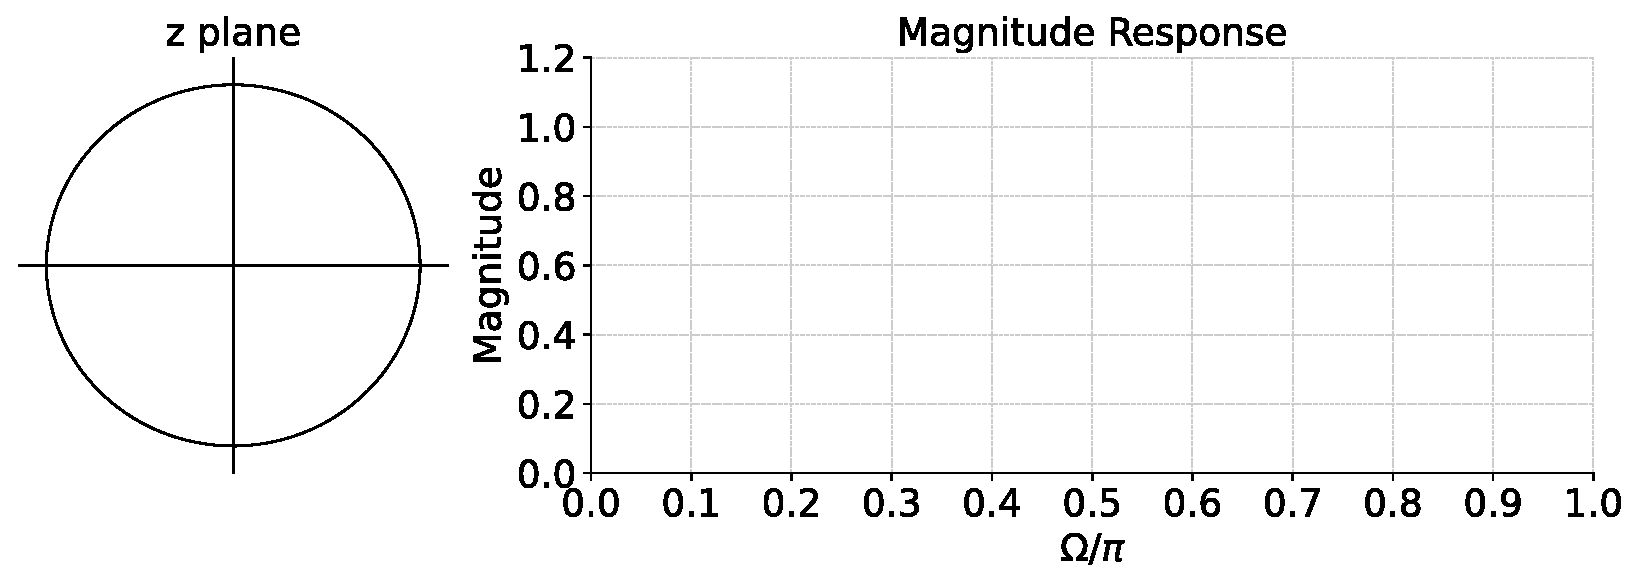
\includegraphics[width=0.7\textwidth]{img/freqpz.eps}
  \end{figure}

  \begin{figure}
  \centering
  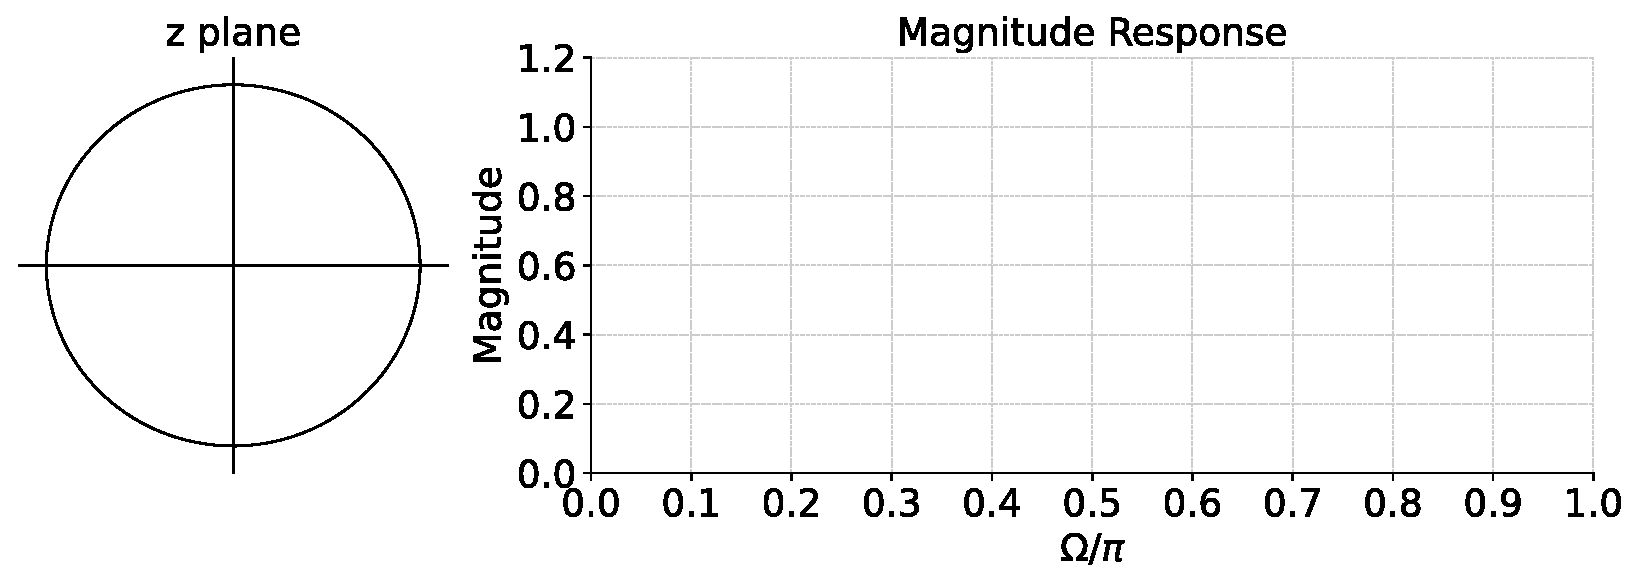
\includegraphics[width=0.7\textwidth]{img/freqpz.eps}
  \end{figure}
  
\end{frame}


\begin{frame}[t]
  \frametitle{Pole-Zero Placement and Frequency Response}
  \[ H(z) = b_0\frac{\lp 1 - z_1z^{-1}\rp \lp 1 - z_2z^{-1}\rp}{\lp 1 - pz^{-1} \rp \lp 1 - p^{*}z^{-1} \rp} \]

  Determine $b_0$, $z_1$, $z_2$, and $p$ to desgin a bandpass filter such that, $H \lp \Omega = 0\rp = 0$ and $H \lp \Omega = \pi \rp = 0$, the center of the passband in at $\Omega = \frac{\pi}{2}$ and $\vert H\lp \Omega = \frac{\pi}{4} \rp \vert = \frac{1}{\sqrt{2}}$.
\end{frame}


\begin{frame}[t]
  \frametitle{FIR and IIR Digital Filter}
  \begin{itemize}
    \item Two types of filters:
    \begin{itemize}
      \item FIR filter: $h[n]$ is of finite length.
      \[ h[n] = 0, \,\, \forall n \neq 0 \quad \text{ and } n > N \]
      \item IIR filter: $h[n]$ is of infinite length.
      \[ h[n] = 0, \,\, \forall n \neq 0 \]
    \end{itemize}
  \end{itemize}
\end{frame}


\begin{frame}[t]
  \frametitle{Linear Phase FIR Filters}

  We will only deal with filter with real impulse response,
  \[ \implies H\lp \Omega \rp = H^*\lp -\Omega \rp, \,\,\, -\pi \leq \Omega < \pi \implies \begin{cases} \vert H\lp \Omega \rp \text{ is an even function of } \Omega \\
  \arg H\lp \Omega \rp \text{ is an odd function of } \Omega \end{cases} \]

  We will only discuss the design of linear phase filters.

  \[  \arg H\lp \Omega \rp = \begin{cases} m \cdot \Omega, & H\lp \Omega  \rp > 0 \\ m \cdot \Omega \pm \pi, & H\lp \Omega \rp < 0 \end{cases} \]
  \vspace{0.1cm}

  Any signal that is symmetric or anti-symmetric with response to some time point will have a linear phase response.
  \vspace{0.25cm}
  % Symmetry impulse response about $n = 0$.
  % \[ h[n] = h[-n] \implies H \lp \Omega \rp \text{ is real.} \7implies \arg H\lp \Omega \rp = \begin{cases} 0, & \H\lp \Omega \rp > 0 \\ \pi, & H\lp \Omega \rp < 0 \]
\end{frame}


\begin{frame}[t]
  \frametitle{Symmetric Impulse Response}
  
  \textbf{Symmetry impulse response} about $n = 0$.
  \[ \begin{split} h[n] = h[-n] & \implies H\lp \Omega \rp = 2 \sum_{n=1}^{\infty} h[n] \cos \lp \Omega n\rp \\ 
      & \implies \arg H\lp \Omega \rp = \begin{cases} 0, & H\lp \Omega \rp > 0 \\ \pi, & H\lp \Omega \rp < 0 \end{cases}
     \end{split}
     \]
  
  \textbf{Anti-symmetry impulse response} about $n = 0$.
  \[ \begin{split} h[n] = -h[-n] & \implies H\lp \Omega \rp = -2j \sum_{n=1}^{\infty} h[n] \sin \lp \Omega n\rp \\ 
      & \implies \arg H\lp \Omega \rp = \begin{cases} -\frac{\pi}{2}, & \Im \lp H\lp \Omega \rp \rp > 0 \\ -\frac{3\pi}{2}, & \Im \lp H\lp \Omega \rp \rp < 0 \end{cases}
     \end{split}
     \]
\end{frame}


\begin{frame}[t]
  \frametitle{Symmetric, Causual, FIR Impulse Response}
  
  Let the length of the impulse response be $M$ (odd). Then, a symmetric, causal impulse response is given by,
  \[ h[n] = h[M - n -1] \implies H\lp \Omega \rp = H_r\lp \Omega \rp e^{j \Theta\lp \Omega \rp}\]
  \[ \Theta\lp \Omega \rp = \begin{cases} -\Omega \lp \frac{M-1}{2}\rp, & H_r\lp \Omega \rp > 0 \\ -\Omega \lp \frac{M-1}{2} \rp + \pi, & H_r\lp \Omega \rp < 0 \\ \end{cases} \]
\end{frame}


\begin{frame}[t]
  \frametitle{Anti-Symmetric, Causual, FIR Impulse Response}
  
  Let the length of the impulse response be $M$ (odd). Then, an anti-symmetric, causal impulse response is given by,
  \[ h[n] = -h[M - n -1] \implies H\lp \Omega \rp = H_r\lp \Omega \rp e^{j \Theta\lp \Omega \rp}\]
  \[ \Theta\lp \Omega \rp = \begin{cases} \frac{\pi}{2} - \Omega \lp \frac{M-1}{2}\rp, & H_r\lp \Omega \rp > 0 \\ \frac{3\pi}{2}  - \Omega \lp \frac{M-1}{2} \rp, & H_r\lp \Omega \rp < 0 \\ \end{cases} \]
\end{frame}


\begin{frame}[t]
  \frametitle{FIR Filter Design: Windowing}
  Window the impulse response of the desired frequency response.
  \[ H_d\lp \Omega \rp \xrightarrow[]{\text{IDTFT}} h_d[n] \xrightarrow[{w[n]}]{\text{Window}} h[n] = w[n] \cdot h_d[n] \xrightarrow[]{\text{DTFT}} H\lp \Omega \rp \approx H_d\lp \Omega \rp \]

  The resulting frequency response $H\lp \Omega \rp$ is,
  \[ H\lp \Omega \rp = H_d\lp \Omega \rp * W\lp \Omega \rp \]

  where, $w[n] \xrightarrow[]{\text{DTFT}} W \lp \Omega \rp$.
\end{frame}


\begin{frame}[t]
  \frametitle{FIR Filter Design: Windowing}
  
  \begin{figure}
  \centering
  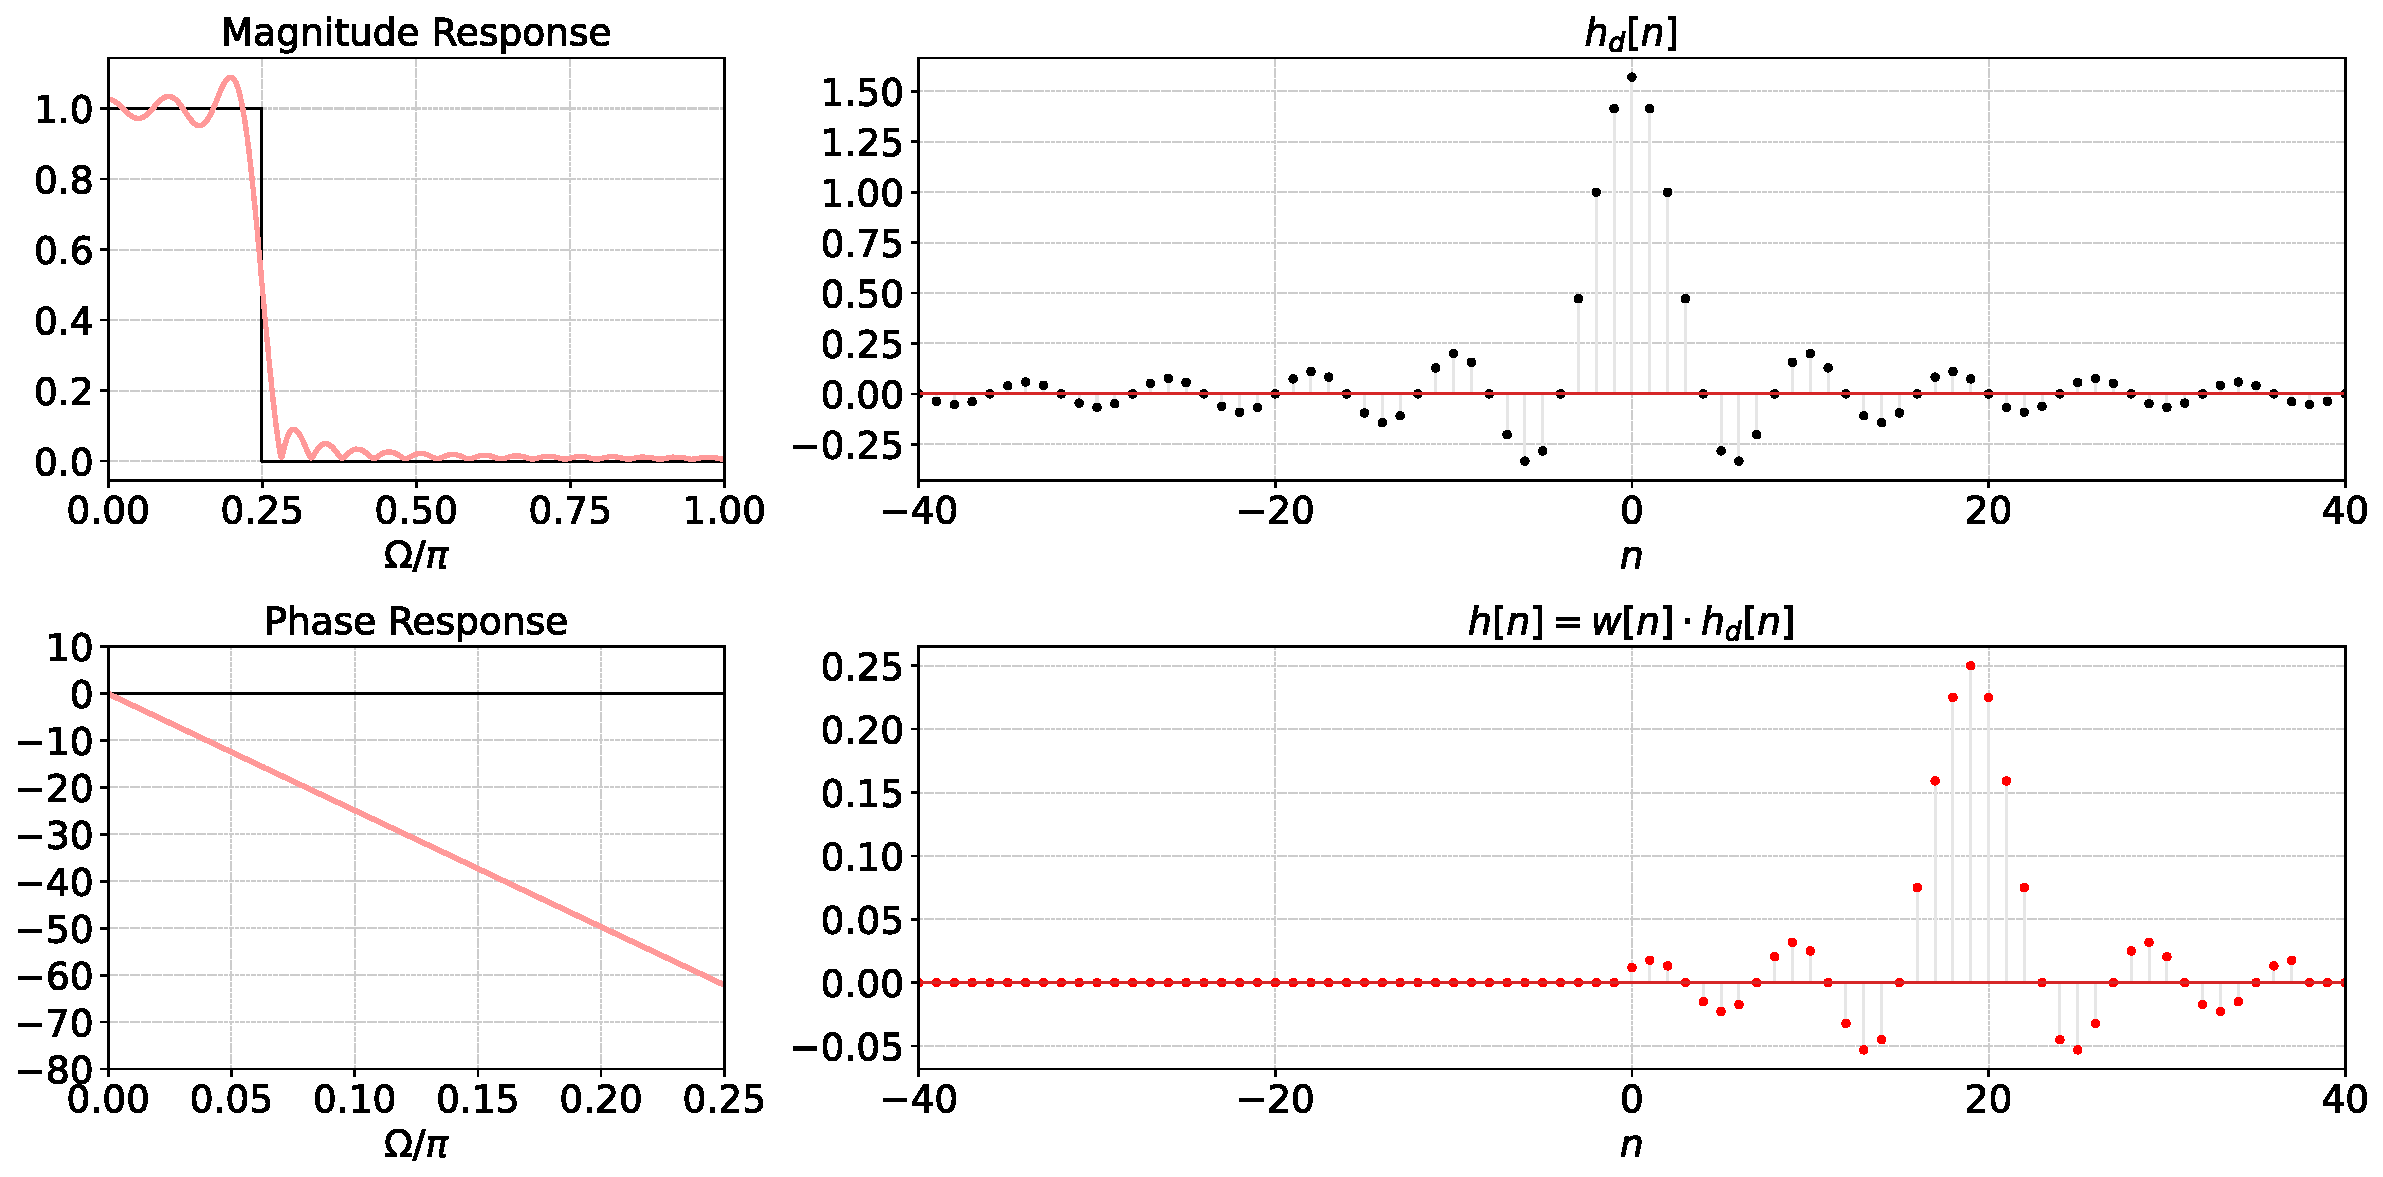
\includegraphics[width=1\textwidth]{img/firwindow.eps}
  \end{figure}

\end{frame}


\begin{frame}[t]
  \frametitle{FIR Filter Design: Windowing}
  
  \begin{figure}
  \centering
  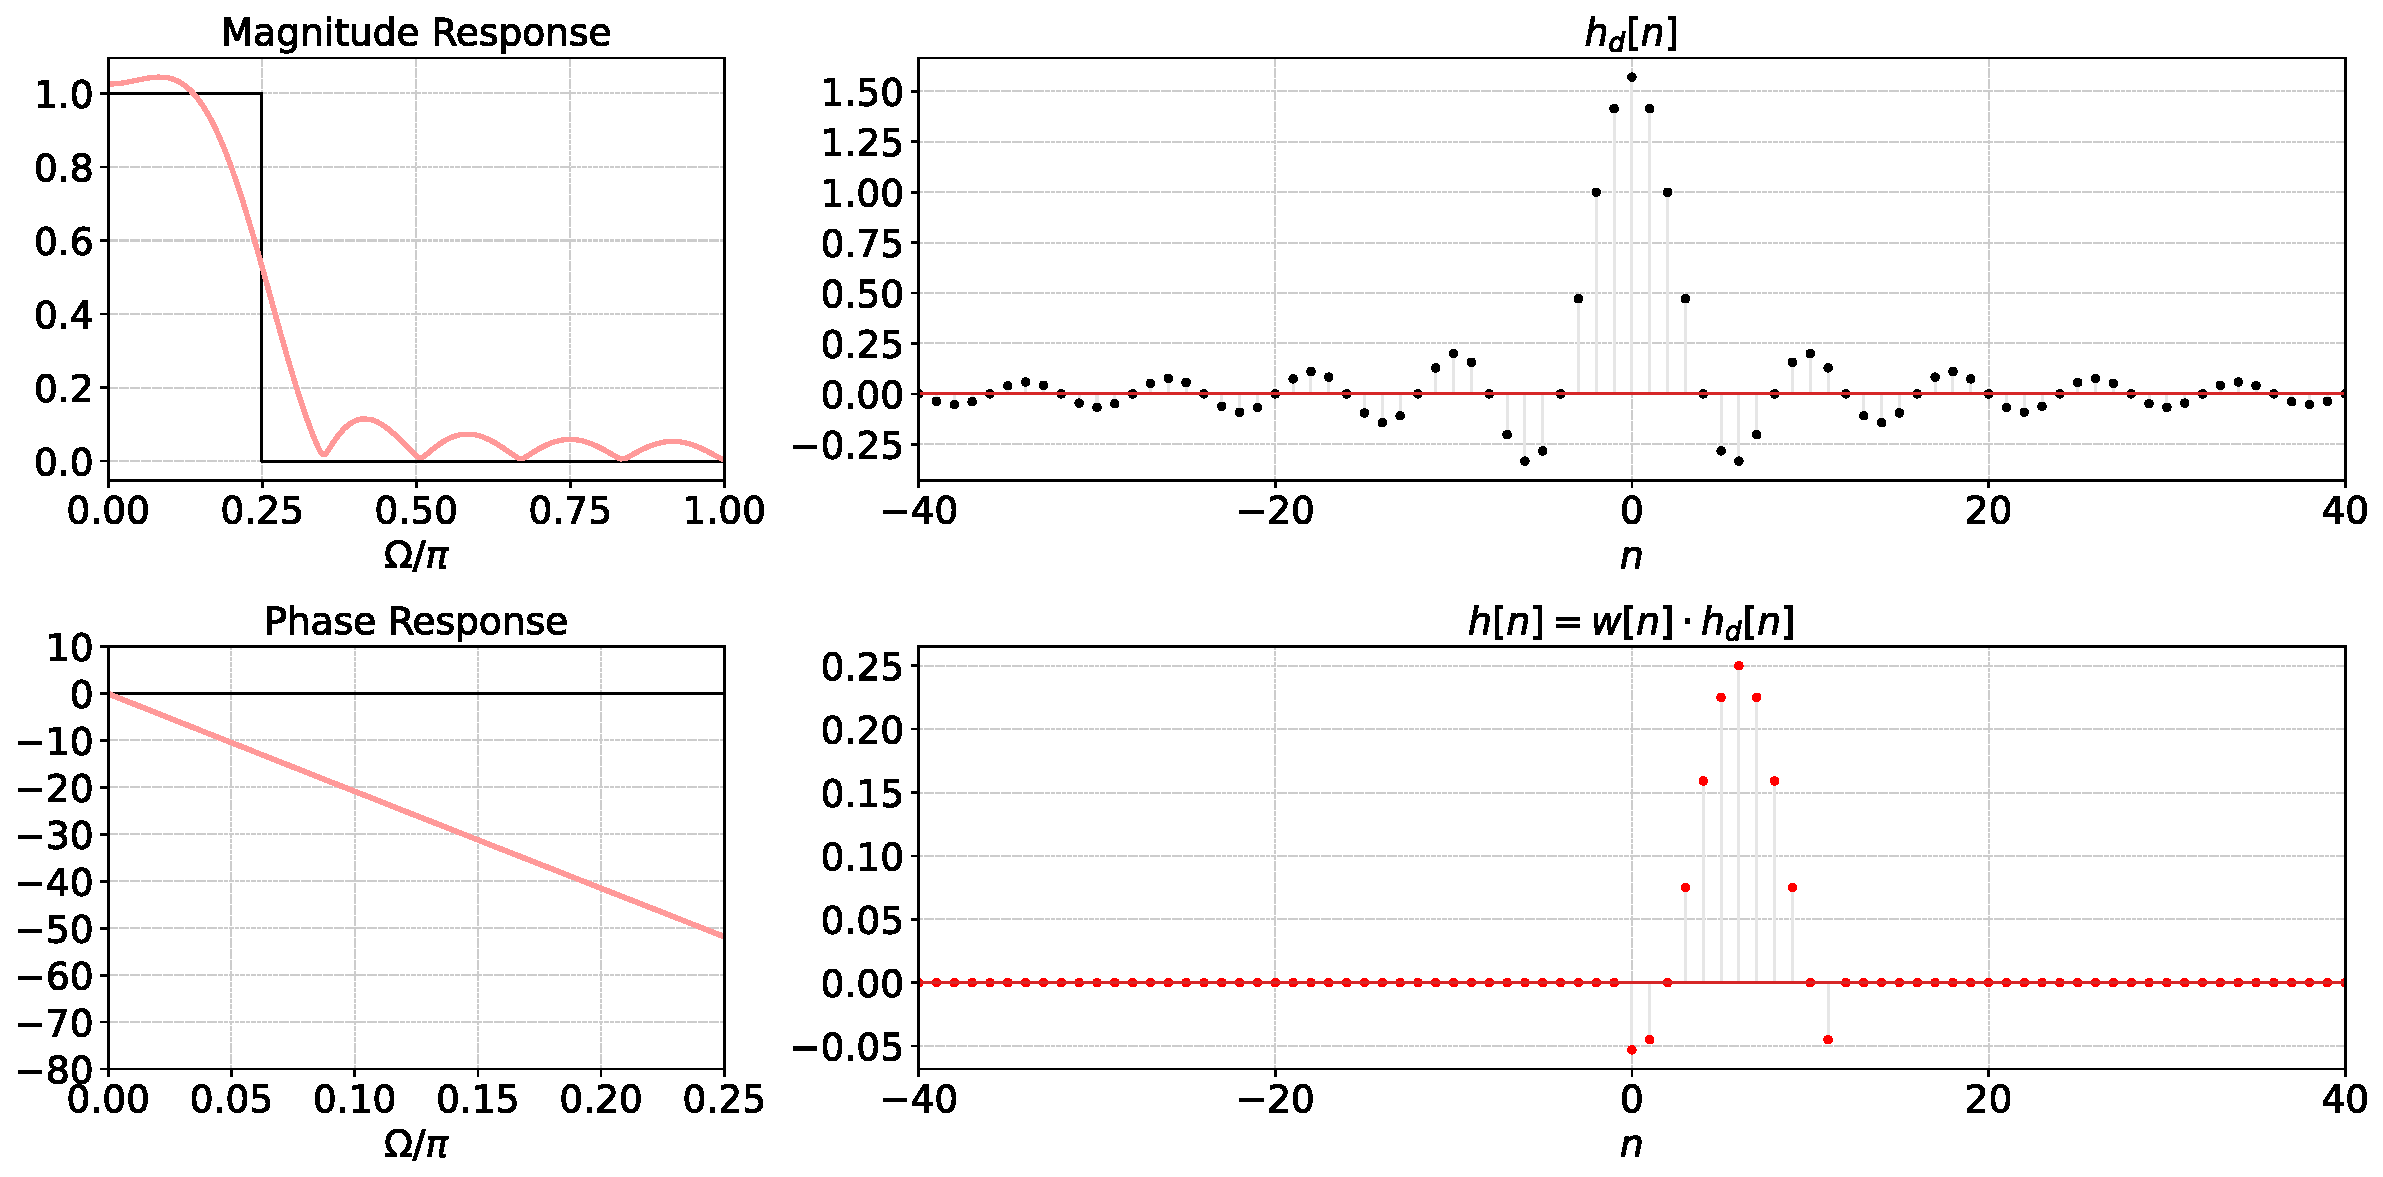
\includegraphics[width=1\textwidth]{img/firwindow2.eps}
  \end{figure}

\end{frame}


\begin{frame}[t]
  \frametitle{FIR Filter Design: Windowing}
  
  \begin{figure}
  \centering
  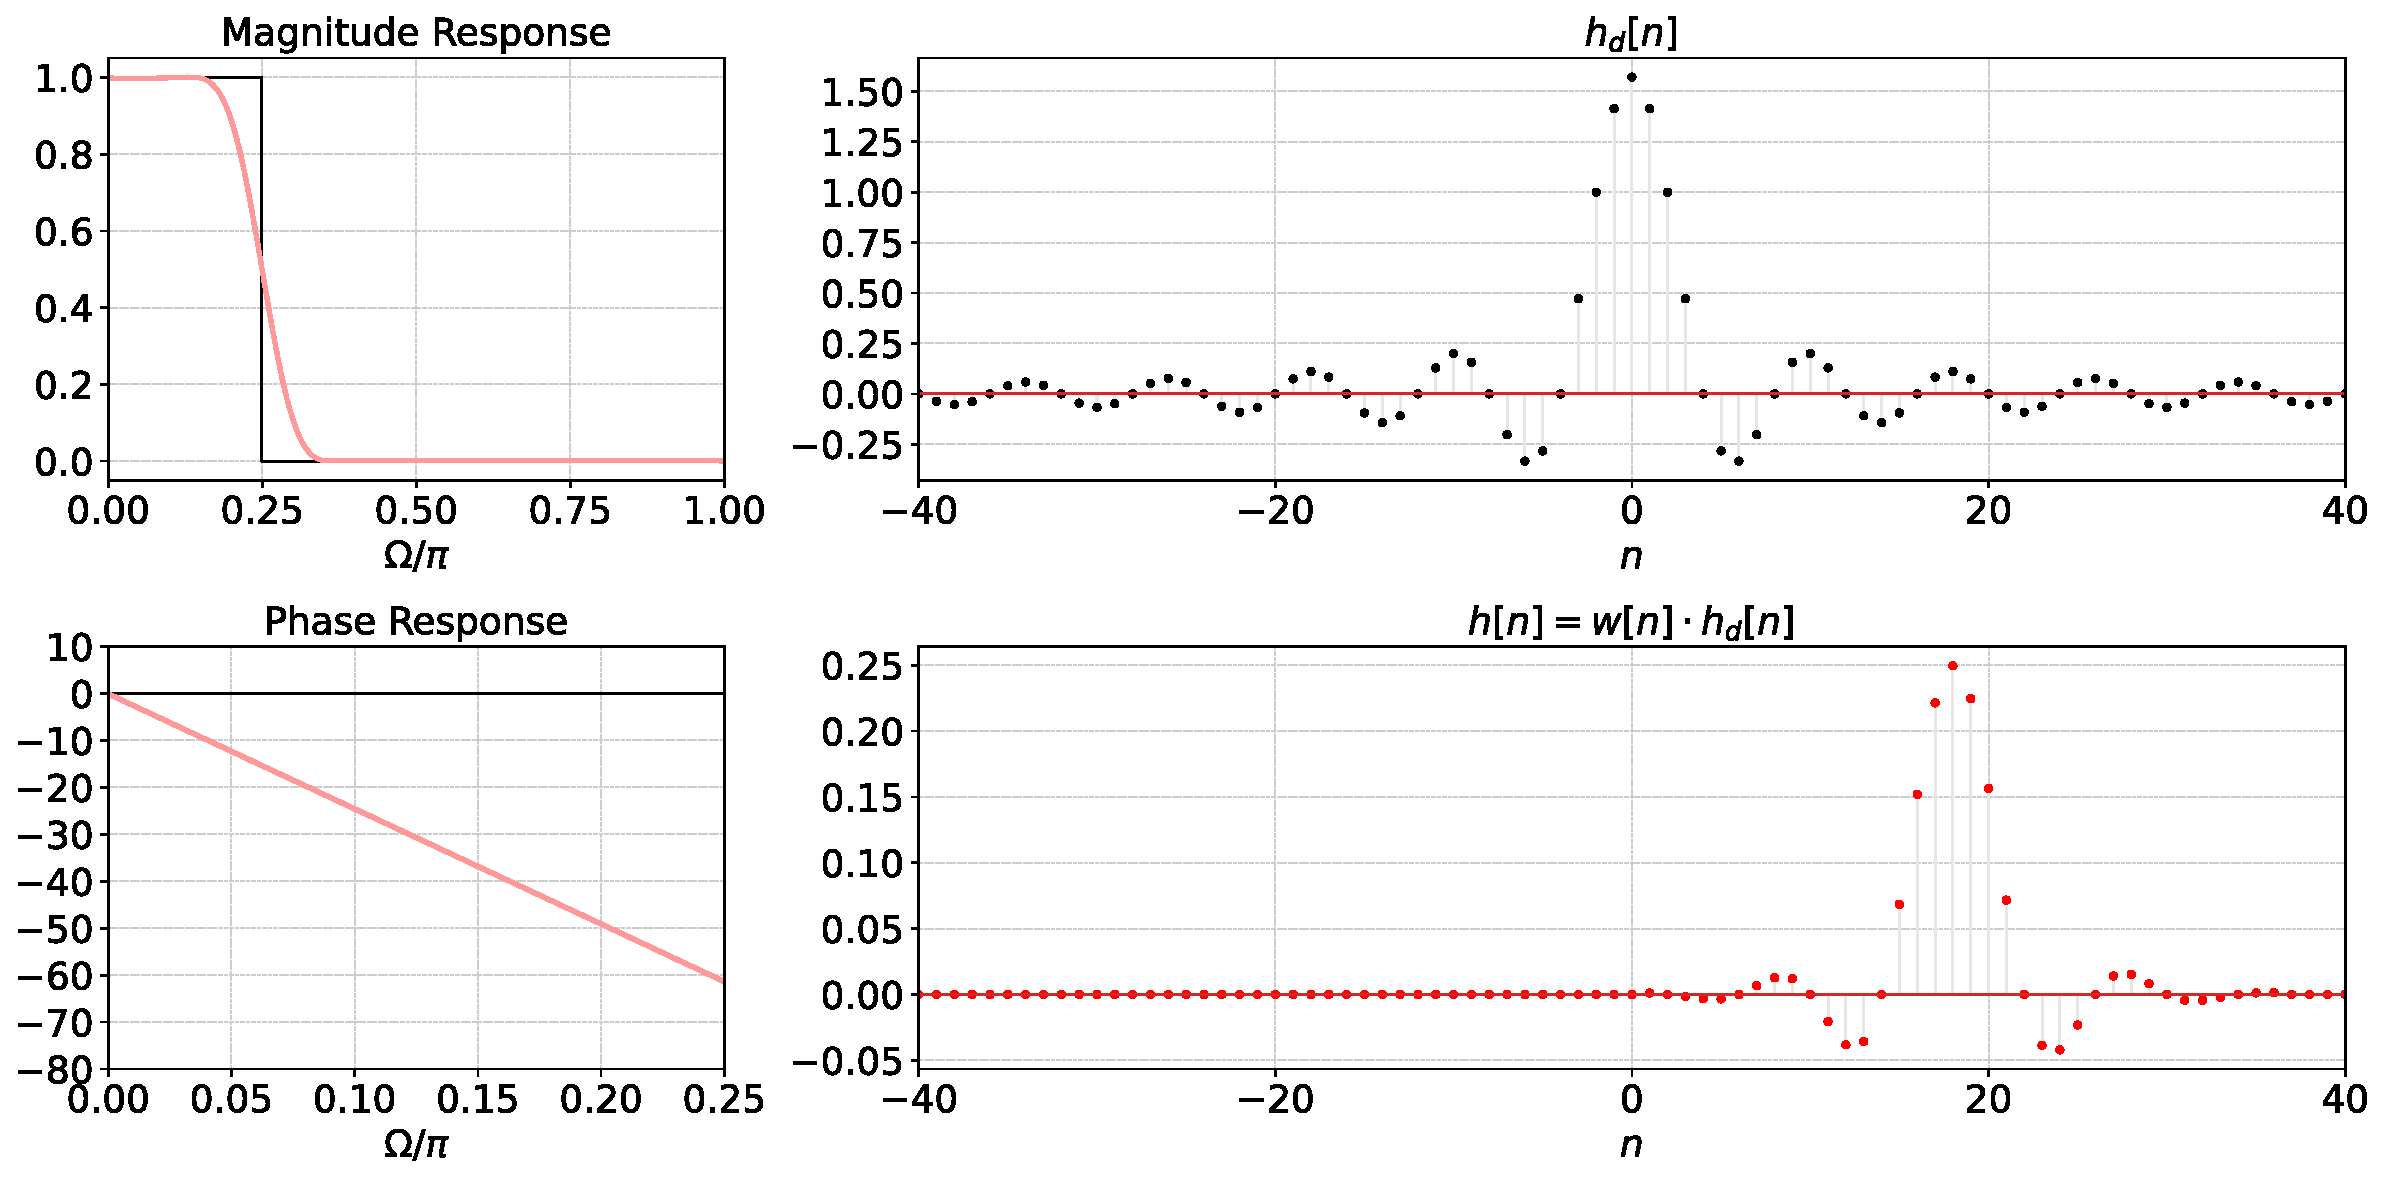
\includegraphics[width=1\textwidth]{img/firwindowhamm.eps}
  \end{figure}

\end{frame}


\begin{frame}[t]
  \frametitle{FIR Filter Design: Windowing}

  \[ H_d\lp \Omega \rp \xrightarrow[]{\text{IDTFT}} h_d[n] \xrightarrow[{w[n]}]{\text{Window}} h[n] = w[n] \cdot h_d[n] \longrightarrow b_i = h[i], \,\, 0 \leq i \leq M \]

\end{frame}


\begin{frame}[t]
  \frametitle{FIR Filter Design: Windowing}
  
  \begin{figure}
  \centering
  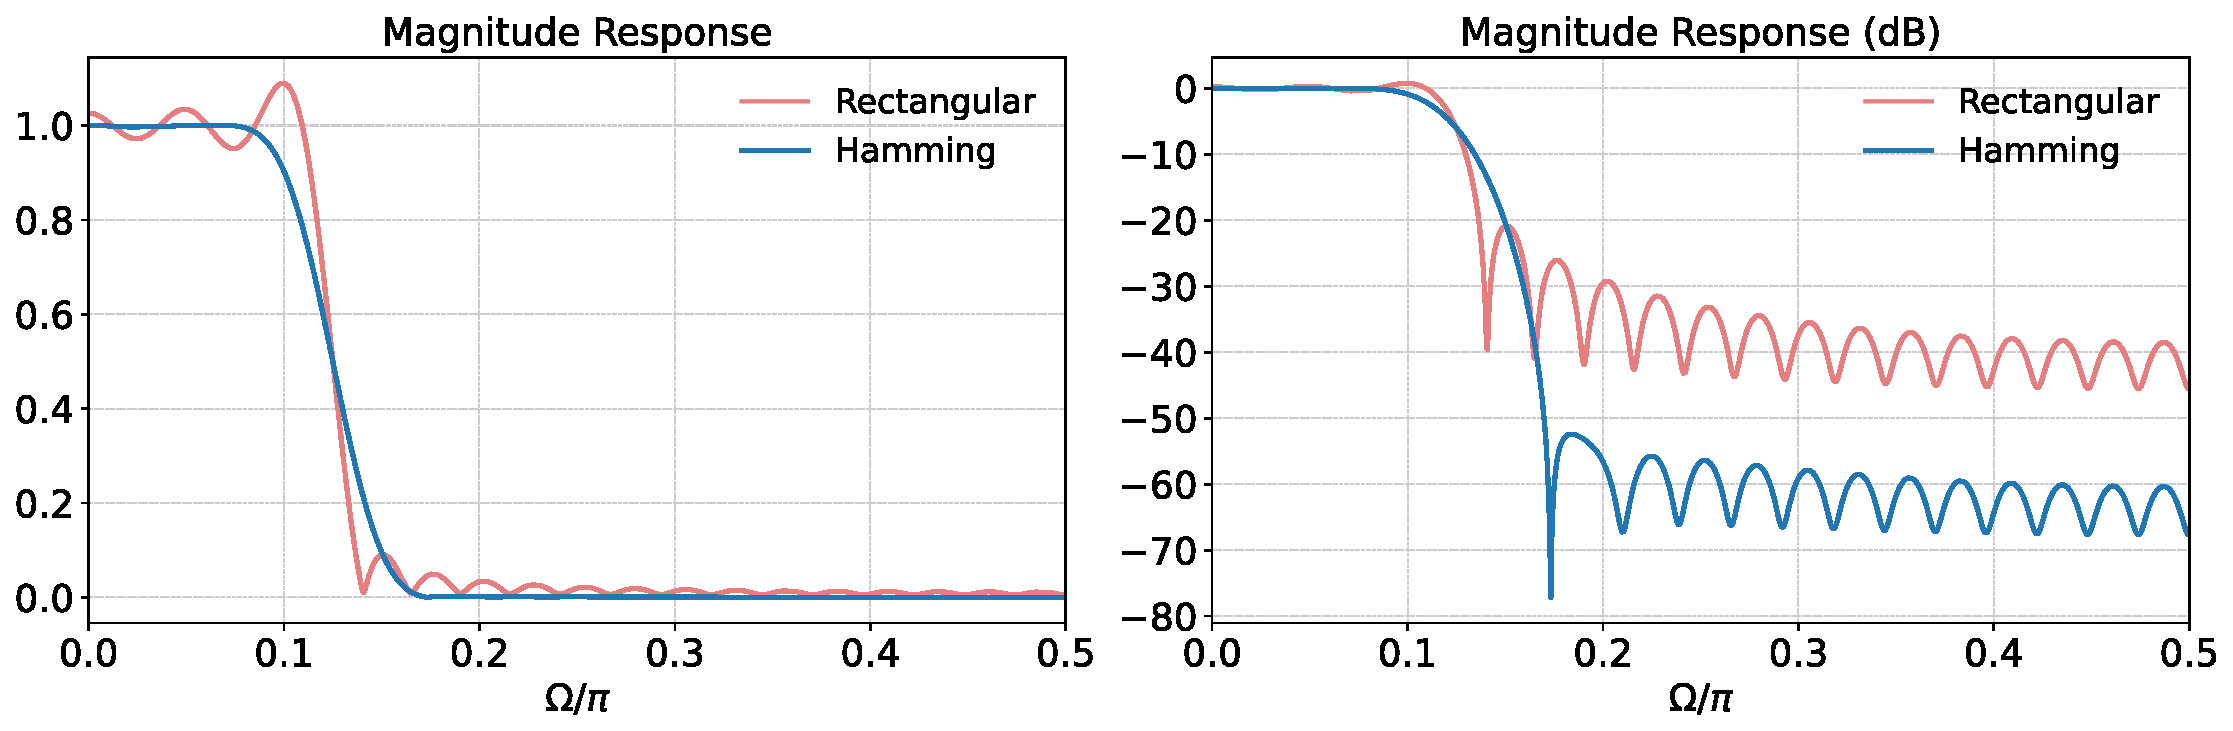
\includegraphics[width=1\textwidth]{img/windowcompare.eps}
  \end{figure}

  Different windows trade-off between the width of the transition band and the level of passband attentuation, and nature of the ripple in the pass and stopbands.
\end{frame}


\begin{frame}[t]
  \frametitle{FIR Filter Design: Frequency sampling}

  We can specify the desired frequency response $H_d\lp \Omega \rp$ at a set of equally spaced frequenceies,
  \[ \Omega_k = \frac{2\pi k}{M}\] 
  
\end{frame}


\begin{frame}[t]
  \frametitle{FIR Filter Design: Frequency sampling}

  \begin{figure}
  \centering
  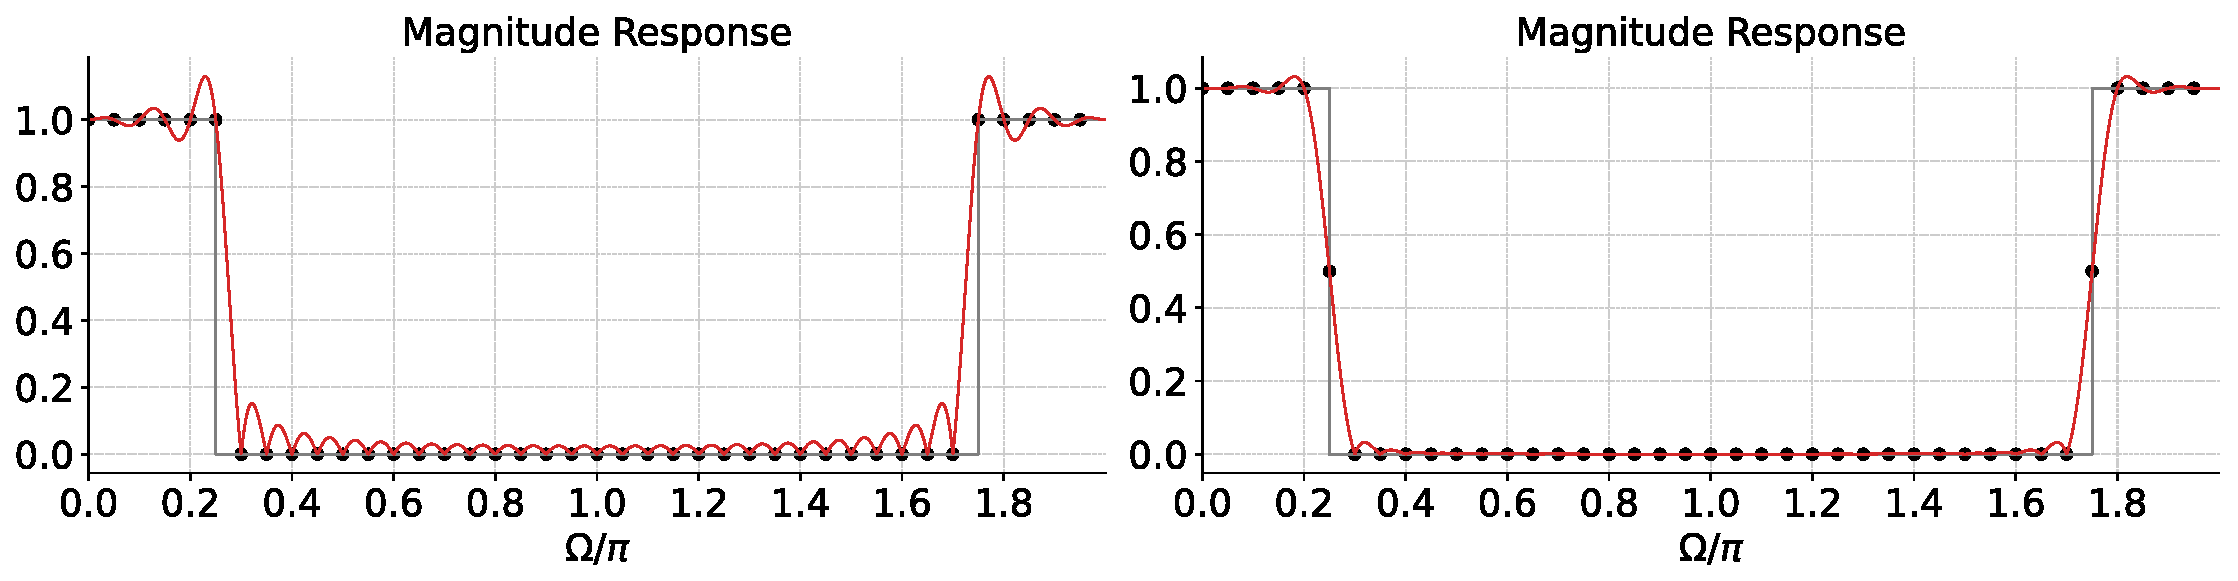
\includegraphics[width=1\textwidth]{img/firfreqsamp.eps}
  \end{figure}

\end{frame}


% \begin{frame}[t]
%   \frametitle{FIR Filter Design}

%   \[ H_d\lp \Omega \rp \xrightarrow[]{\text{IDTFT}} h_d[n] \xrightarrow[{w[n]}]{\text{Window}} h[n] = w[n] \cdot h_d[n] \longrightarrow b_i = h[i], \,\, 0 \leq i \leq M \]

% \end{frame}


\begin{frame}{FIR Filter Design}
  Advantages of FIR filters:
  \begin{itemize}
    \item Always stable. $\sum_n \vert h[n] \vert < \infty$
    \item Linear phase $\implies$ No phase distortion.
  \end{itemize}
  \vspace{1cm}

  Disadvantages of FIR filters:
  \begin{itemize}
    \item Same specs might require a longer filter.
    \item Might requires iterative numerical procedures for design.
  \end{itemize}
  \vspace{1cm}
\end{frame}


\begin{frame}[t]
  \frametitle{IIR Filter Design}

  We are intersted in causal systems that have rational transfer functions,
  \[ H(z) = \frac{B(z)}{A(z)} \longrightarrow y[n] = \sum_{k=1}^M b_k \cdot x[n - k] - \sum_{l=1}^N a_l \cdot y[n - l] \] 
  
  Most popular approach is to design a analog filter and then translate it into a corresponding digital filter.

  \[ \text{Digital filter specs} \longrightarrow \text{Analog filter specs} \longrightarrow \text{Analog filter } H_a(s) \]

  \[ \text{Analog filter } H_a(s) \xrightarrow[\text{transformation}]{\text{Bilinear}} \text{Digital filter } H(z) \]

  \textbf{Bilinear transformation}: Substitute $s = \frac{2}{T}\frac{1 - z^{-1}}{1 + z^{-1}}$.
  \[ H\lp z \rp = H_a\lp s \rp \bigg\vert_{s = \frac{2}{T}\frac{1 - z^{-1}}{1 + z^{-1}}} \]
\end{frame}


\begin{frame}[t]
  \frametitle{IIR Filter Design}

  Analog to digital Frequency mapping done by the bilinear transformation.
  \[ \omega = \frac{2}{T} \tan \lp \frac{\Omega}{2} \rp \implies  \Omega = 2 \tan^{-1} \lp \frac{\omega T}{2} \rp \]

  \begin{figure}
  \centering
  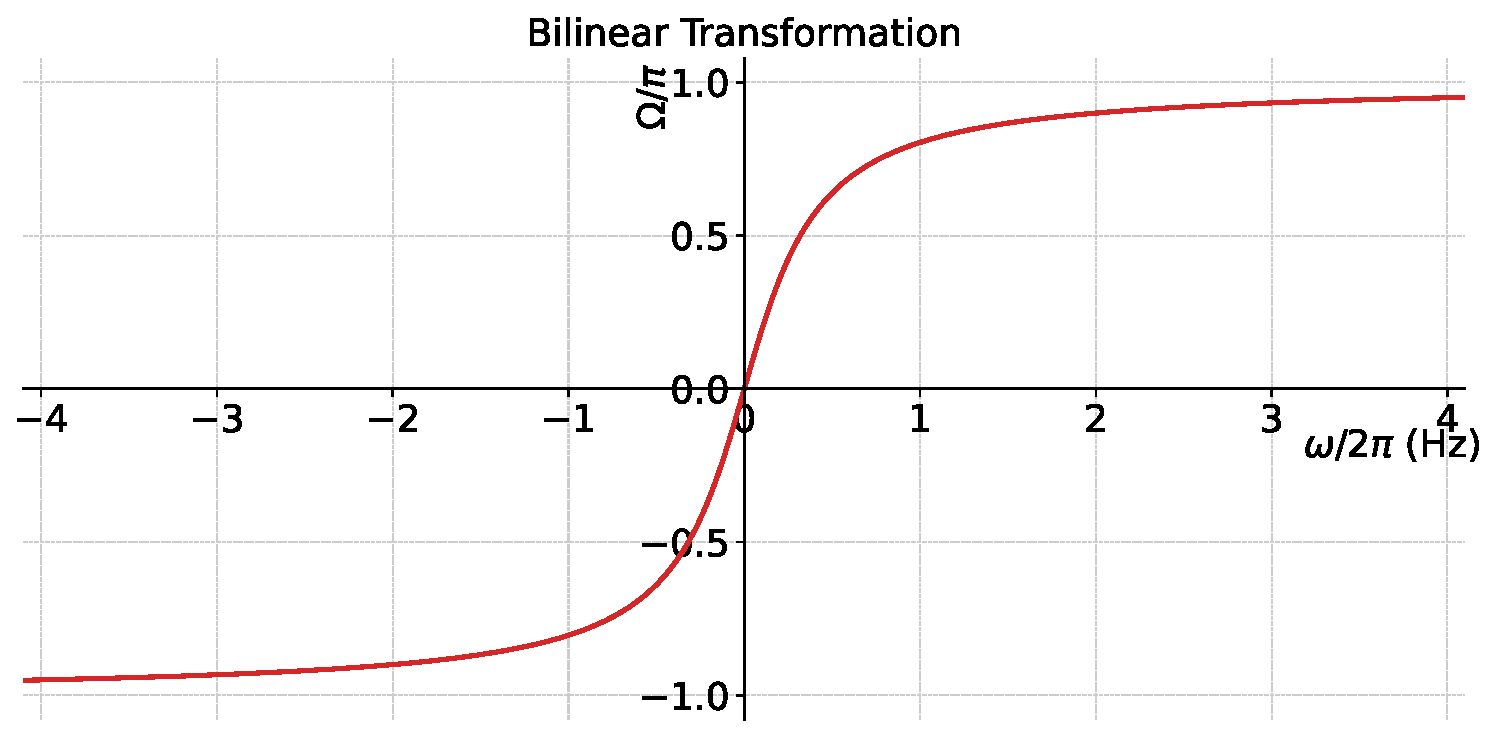
\includegraphics[width=0.7\textwidth]{img/bilintrans.eps}
  \end{figure}
\end{frame}


\begin{frame}[t]
  \frametitle{IIR Filter Design}
  \begin{figure}
  \centering
  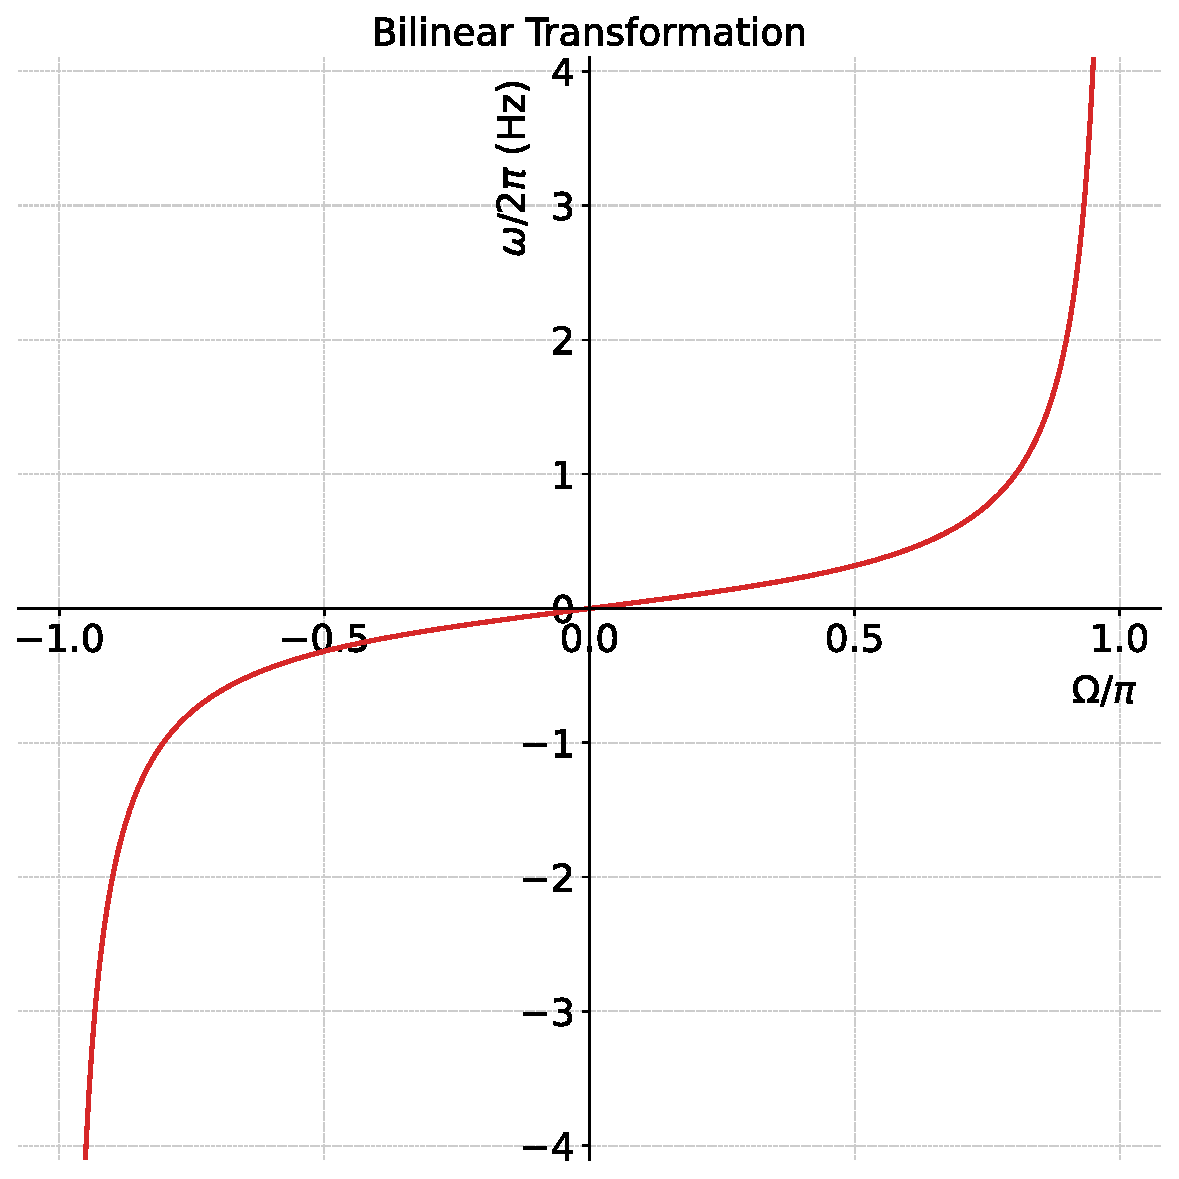
\includegraphics[width=0.45\textwidth]{img/bilintransinv.eps}
  \end{figure}
\end{frame}


\begin{frame}[t]
  \frametitle{IIR Filter Design}
  \begin{figure}
  \centering
  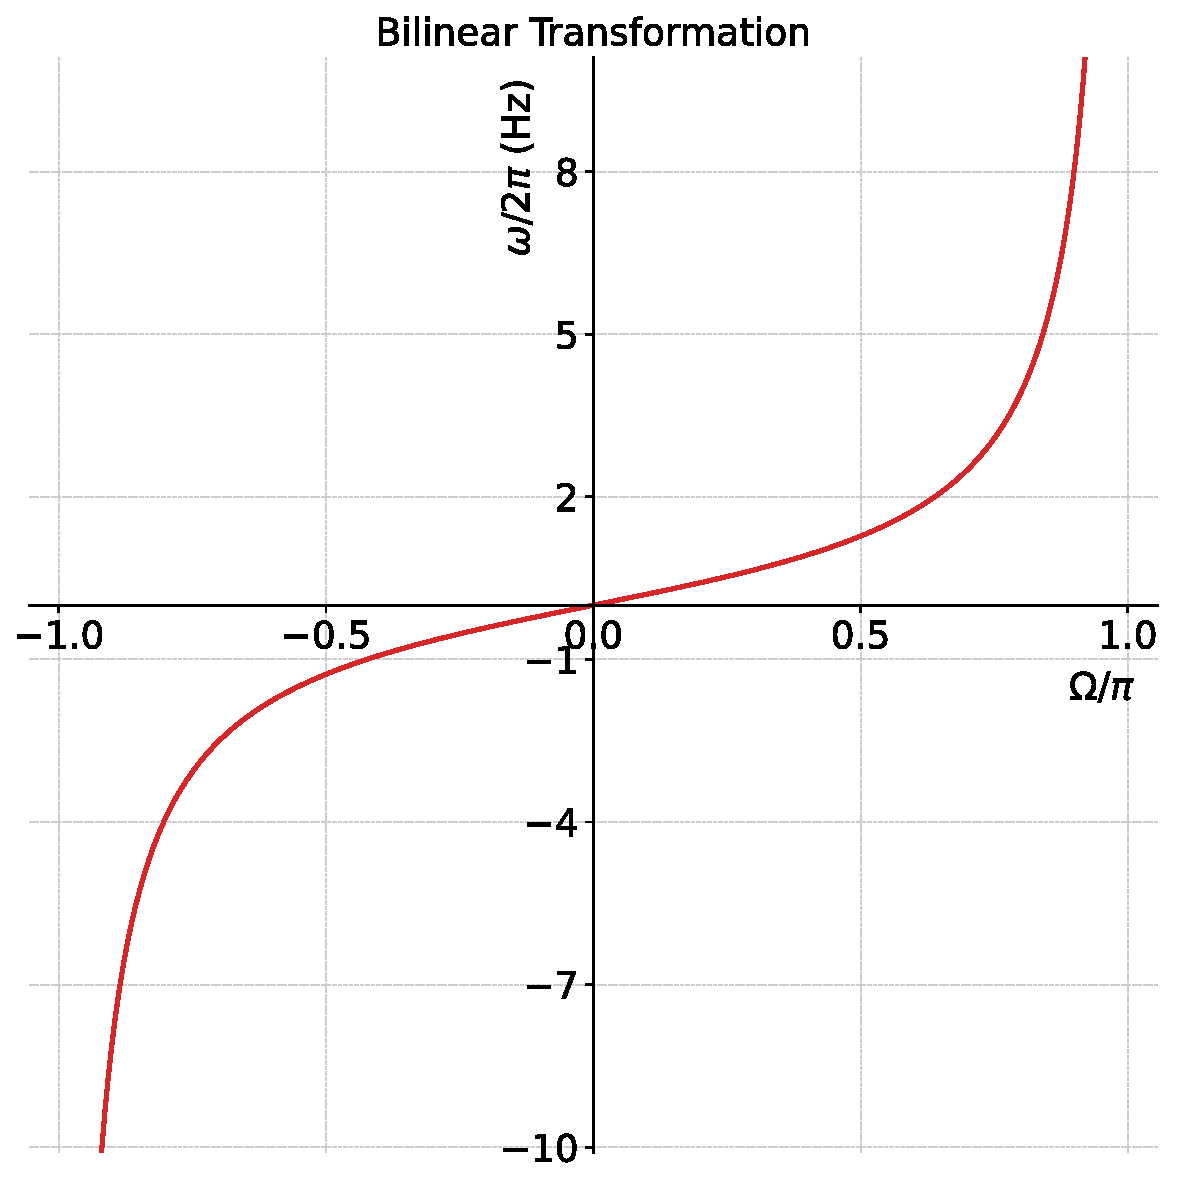
\includegraphics[width=0.5\textwidth]{img/bilintransinv2.eps}
  \end{figure}
\end{frame}


\begin{frame}{IIR Filter Design}
  Advantages of IIR filters:
  \begin{itemize}
    \item Requires lower number of parameters than FIR.
    \item Design using analog filter design tools.
  \end{itemize}
  \vspace{1cm}

  Disadvantages of IIR filters:
  \begin{itemize}
    \item Can be unstable.
    \item More sensitive to round-off errors.
  \end{itemize}
  \vspace{1cm}
\end{frame}

\end{document}